% !TEX root = /home/frank/School/thesis_text/thesis.tex




\chapter{Introduction} 
Up until halfway the first decade of the new millennium it was possible to gain computing performance whilst also being able to maintain the sequential programming paradigm. This was due to Moore's law, stating that the number of transistors on integrated circuits double approximately every two years. There was no need for research into explicit parallelism because the next generation of computing devices was just around the corner. This new generation would increase the performance with zero effort required from the programmer.To perpetuate the sequential programming paradigm several innovations such as multiple issue, deep pipelines and out of order execution were introduced. These optimizations  were inefficient in both the use of transistors and power. Eventually it became impossible to progress any further whilst still supporting the sequential paradigm. The integrated circuit industry was unable to continue decreasing the size of MOSFETs whilst continuing to increase the clock frequency. The industry had hit what is called the power wall.
The solution to this problem was to turn to parallel processors, meaning that there is more than one processing unit working at a time. A lot of real world applications are parallel, and hardware can be made parallel with relative ease. The problem lies in the programming model, how to exploit this parallelism and make programming for these parallel architectures easier and transparent for the programmer.



\section{Computing Components}

\subsection{Multicore Processor}
The multicore processor is the solution presented for the aforementioned problems by the traditional CPU manufacturers such as Intel and AMD. The idea behind this type of processor is to place a number of cores (currently up to eight) on the same die. This presents a compromise between maintaining sequential performance whilst also providing a certain advantage of parallel processing. Parallel programming for these processors presents certain challenges, whilst their modest parallelism cannot provide a dramatic improvement in power performance. Multicore processors are unlikely to be a one-size-fits-all solution to the parallel problem.\cite{asanovic_landscape_????}

\subsection{Graphics Processing Units} 
Graphics processing units are a type of coprocessor used in traditional computers to process images for output to the display. However recently there has been an increased interest in the GPGPU, a general purpose graphics processing unit. These processors implement a different paradigm, namely the manycore paradigm. A  GPU is a processor with hundreds single instruction multiple data cores, each of which is heavily multi-threaded. Because of this large amount of cores the FLOPS (floating point operations per second) is unrivaled\cite{kirk_programming_2010}. GPU's, due to their SIMD (single instruction multiple data) nature present some problems, conditional execution paths for example, present a serious overhead on the GPU. GPU's are programmed with either OpenCL (open standard) or CUDA (proprietary to Nvidia)

\subsection{Field Programmable Gate Array} 
FPGAs are devices containing a vast amount of configurable logic linked by programmable connections. This logic is comprised of lookup tables (LUTs) grouped together into configurable logic blocks. Any combinatorial function can be programmed into these LUT's. Next to these uncommitted logic blocks a typical FPGA also contains several blocks with a specific function such as block ram and DSP multipliers. FPGAs are an interesting competitor in the parallel processing field because they are not constrained by the Von Neuman architecture. FPGAs follow the dataflow paradigm in which the data \emph{flows} through the logic. Implementing a data-flow is inherently parallel. The different stages in the datapath can also be made effectively sequential making the datapath a pipeline. The fine grained nature of FPGAs also means that the bitwidth can be adapted to the application.


\section{Berkeley dwarfs }

Image processing algorithms are very compute intensive. These makes them prime targets for exploiting parallelism and implementing them on parallel architectures. Which platform is the best fit is dependent on both the algorithm and the data. A common method to subdivide parallel algorithms is presented in , the so called \emph{dwarfs}. These 13 dwarfs are classes of algorithms in which the membership is defined by a similarity in computation and data movement.These 13 dwarfs are classes of algorithms in which the membership is defined by a similarity in computation and data movement.
The dwarfs are:

\begin{multicols}{2}
\begin{enumerate}
\item Dense Linear Algebra
\item Sparse Linear Algebra
\item Spectral Methods
\item N-Body Methods
\item Structured Grids
\item Unstructured Grids
\item MapReduce
\item Combinational Logic
\item Graph Traversal
\item Dynamic Programming
\item Backtrack and Branch-and-Bound
\item Graphical Models
\item Finite State Machines
\end{enumerate}
\end{multicols}

A thorough review of these dwarfs and what kind of computation and communication they entail goes beyond the scope of this document. An updated view can be found in \cite{asanovic_view_2009}.\
Finding out which platform is most suited for a dwarf is a labor intensive task. In \cite{inta_chimera:_2012} a theoretical analysis of dwarf performance on different accelerators in heterogeneous systems is given. A first point of note is that GPGPU's are unsurpassed in floating point arithmetic. Fixed point numbers are a way to overcome this problem. Another point to note is that conditional elements and  costly communication can wreak havoc on the accelerator's performance. In Figure \ref{img:venndiagram_chimera} the analysis is represented by a Venn diagram. In this diagram `*' denotes fixed point operations whilst `\^{}' denotes floating point operations.

\begin{figure}[H]
\centering
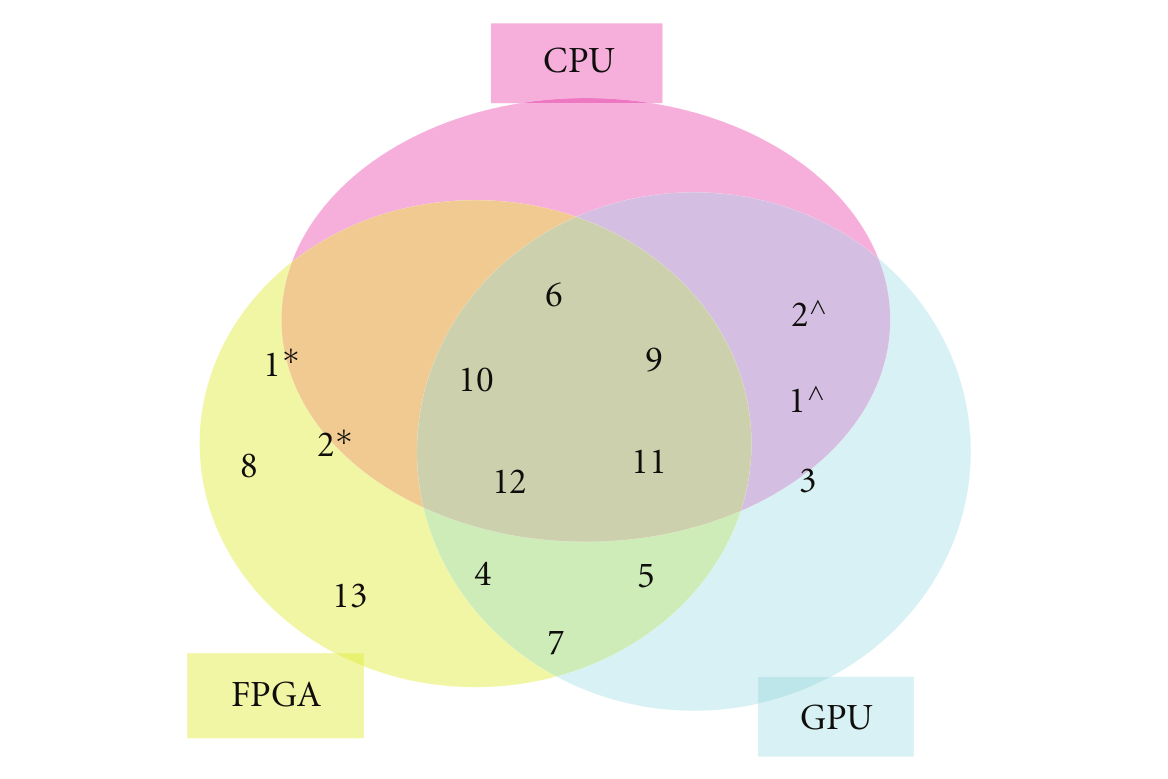
\includegraphics[scale=0.34]{/home/frank/School/thesis_text/images/venndiagram_chimera.png}
\caption{Analysis of different hardware accelerators in regards to performance on a certain dwarf \cite{inta_chimera:_2012} }
\label{img:venndiagram_chimera}
\end{figure}


\section{GUDI Project}

This thesis is inspired by the work of the GUDI project. GUDI is an acronym for \quotationmarks{A Combined \textbf{G}P-GP\textbf{U}/FPGA \textbf{D}esktop for accelerating \textbf{I}mage processing applications}. The research starts from the observation that there is a large need for computing power to process data using computationally intensive image processing algorithms. Conventional Off-the-shelf Desktop computers don't have the necessary processing power to satisfy this demand. A lot of image processing algorithms exhibit parallelism which can be exploited by the right architecture. Two such massively-parallel architectures are GP-GPU's and FPGA's. The GUDI project's goal is to investigate the possibilities and limitations of a computer with such a heterogeneous architecture. It is an investigation into the technologies and development tools and their performance in different situations. The means through which this is done is through the implementation and performance measurement of algorithms. The ultimate goal is to split an algorithm into several parts, executed on the technology (CPU,GPU,FPGA) most fit for the job so as to ensure optimal speed-ups.




